\chapter{Introduzione}
\section{ Premessa }

\textbf{Def - Sistemi dinamici:}  sono un'evoluzione temporale di un ingresso e un'uscita, vengono modellati dalle \textbf{equazioni differenziali}.\\
Vedremo sono funzioni monodimensionali (cioè dipendenti solo dal tempo) ma in realtà possiamo benissimo avere più dimensioni.\\
I modelli ci danno una stima del comportamento di una sistema, in particolare il modello delle equazioni differenziali si può svolgere: nel tempo, nel dominio della trasformata di Laplace (utile con i segnali esponenziali e sinusoidali) e nel dominio della trasformata di Fourier (è un restrizione di Laplace, è utile nei segnali sinusoidali).\\
Studieremo le proprietà dei sistemi, di queste la più importante è la stabilità.\\
\textbf{Modelliamo un sistema} come fosse una scatola nera, avrà un segnale come input e output (es. suono 1D, immagine 2D).\\
I sistemi ci servono per vari motivi: possono facilitare la trasmissione di un segnale, migliorarlo accentuando alcune informazioni o eliminandone altre (filtraggio).\\
Vogliamo vedere i sistemi come \textbf{funzioni matematiche} (pag. 69 libro "")\\

\begin{figure}
	\centering
	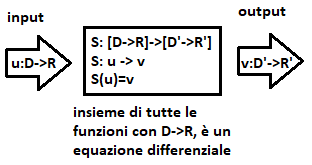
\includegraphics[width=0.7\linewidth]{sistema}
	\caption{ modello di un sistema come scatola nera}
	\label{fig:sistema}
\end{figure}



$ \forall s \in D' $ allora $ v(s)=(S(u))(s)\in R'  $ \\

\pagebreak

Abbiamo tre tipi di sistemi:\\
- Continui: operano su segnali continui\\
- Discreti: operano su segnali discreti\\
- Ibridi fra continui e discreti (non li vedremo)\\

\begin{figure}[h]
	\centering
	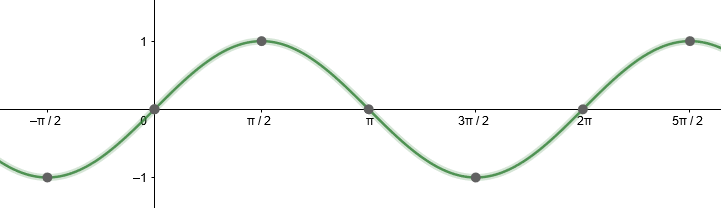
\includegraphics[width=0.7\linewidth]{seno}
	\caption{Segnale continuo}
	\label{fig:seno}
\end{figure}


\begin{figure}[h]
	\centering
	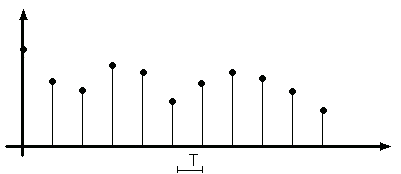
\includegraphics[width=0.7\linewidth]{tempo_discreto}
	\caption{ Segnale discreto}
	\label{fig:tempodiscreto}
\end{figure}

\textbf{Quantizzazione e campionamento}\\
Per andare da analogico a digitale (A->D) ho bisogno di campionamento e quantizzazione.\\

Campionamento: trasformiamo il dominio. Non ho sempre perdita di dati.\\

\begin{figure}[h]
	\centering
	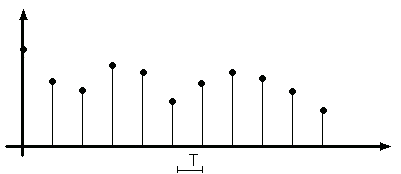
\includegraphics[width=0.7\linewidth]{tempo_discreto}
	\caption{ Segnale campionato nel tempo}
	\label{fig:tempodiscreto}
\end{figure}

\pagebreak
Quantizzazione: trasformiamo il codominio. Ha sempre perdita di informazione.\\

\begin{figure}[h]
	\centering
	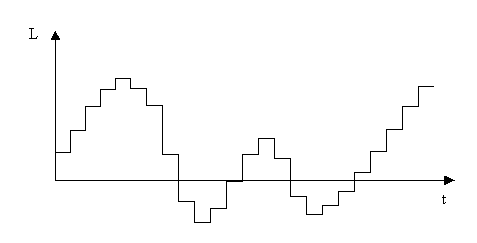
\includegraphics[width=0.7\linewidth]{quantizzato}
	\caption{ Segnale sinusoidale quantizzato nelle ampiezze}
	\label{fig:quantizzato}
\end{figure}

\textbf{Sistemi LTI}\\
Studiamo un tipo particolare di sistemi, che hanno due proprietà: linearità e tempo invarianza (L=lineari, TI=tempo invarianti).\\
- Linearità:\\
Se $ v_{1}=S(u_{1}) $ e $ v_{2}=S(u_{2})  $ 
allora $ S(\alpha u_{1} + \beta u_{2}) 
= \alpha S(u_{1}) + \beta S(u_{2})
= \alpha v_{1} + \beta v_{2} $ con $ \alpha , \beta \in C^{*} $ \\
Oppure grazie al \textbf{principio di sovrapposizione degli effetti} ( stabilisce che per un sistema dinamico lineare l'effetto di una somma di perturbazioni in ingresso è uguale alla somma degli effetti prodotti da ogni singola perturbazione): \\
$ S( \sum_{i=0}^n \alpha_i u_i ) 
=  \sum_{i=0}^n \alpha_i S( u_i )
$ \\
La linearità è dovuta alle equazioni differenziali, all'interno hanno la derivata prima che è essa stessa lineare.\\
- Tempo invariante:\\
 Significa che l'uscita non dipende esplicitamente dal tempo, cioè se un ingresso x(t) produce l'uscita y(t) allora per ogni ingresso traslato $x(t+ \delta )$ si ha un'uscita traslata dello stesso fattore $y(t+ \delta )$.\\
 
 $u(t+ t_0 ) \rightarrow v(t+ t_0 )$
 
\begin{figure}[h]
	\centering
	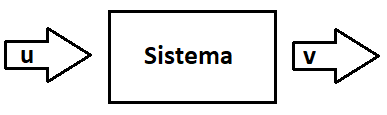
\includegraphics[width=0.7\linewidth]{sistema2}
	\caption{ Sistema generico }
	\label{fig:sistema2}
\end{figure}

\begin{figure}[h]
	\centering
	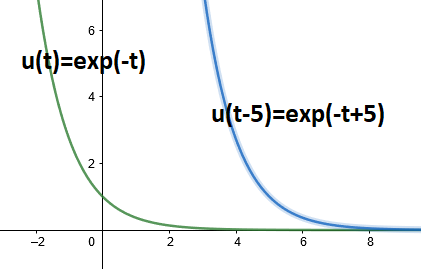
\includegraphics[width=0.7\linewidth]{esponenziale}
	\caption{ Esempio di tempo invariante }
	\label{fig:esponenziale}
\end{figure}


gniiiii
% TODO: eq diff a coefficienti costanti

\pagebreak

\section{ Ripasso sui numeri complessi }